\documentclass[12pt,letterpaper]{article}
\usepackage[utf8]{inputenc}
\usepackage[spanish]{babel}
\usepackage{graphicx}
\usepackage[left=2cm,right=2cm,top=2cm,bottom=2cm]{geometry}
\usepackage{graphicx} % figuras
% \usepackage{subfigure} % subfiguras
\usepackage{float} % para usar [H]
\usepackage{amsmath}
%\usepackage{txfonts}
\usepackage{stackrel} 
\usepackage{multirow}
\usepackage{enumerate} % enumerados
\renewcommand{\labelitemi}{$-$}
\renewcommand{\labelitemii}{$\cdot$}
% \author{}
% \title{Caratula}
\begin{document}

% Fancy Header and Footer
% \usepackage{fancyhdr}
% \pagestyle{fancy}
% \cfoot{}
% \rfoot{\thepage}
%

% \usepackage[hidelinks]{hyperref} % CREA HYPERVINCULOS EN INDICE

% \author{}
\title{Caratula}

\begin{titlepage}
\begin{center}
\large{UNIVERSIDAD PRIVADA-DE-TACNA}\\
\vspace*{-0.025in}
\begin{figure}[htb]
\begin{center}

\includegraphics[width=8cm]{./Imagenes/logo}
\end{center}
\end{figure}
\vspace*{0.15in}
INGENIERIA DE SISTEMAS  \\

\vspace*{0.5in}
\begin{large}
TITULO:\\
\end{large}

\vspace*{0.1in}
\begin{Large}
\textbf{INFORME DE LABORATORIO No 03 -  Creando un Cubo Multimensional con SQL Server
Analysis Services}\\
\end{Large}

\vspace*{0.3in}
\begin{Large}
\textbf{CURSO:} \\
\end{Large}

\vspace*{0.1in}
\begin{large}
INTELIGENCIA DE NEGOCIOS\\
\end{large}

\vspace*{0.3in}
\begin{Large}
\textbf{DOCENTE(ING):} \\
\end{Large}

\vspace*{0.1in}
\begin{large}
 Patrick Cuadros Quiroga\\
\end{large}

\vspace*{0.2in}
\vspace*{0.1in}
\begin{large}
Estudiante: \\ 
Sharon Sosa Bedoya          (2016054460) \\
\end{large}
\end{center}

\end{titlepage}


\tableofcontents % INDICE
\thispagestyle{empty} % INDICE SIN NUMERO
\newpage
\setcounter{page}{1} % REINICIAR CONTADOR DE PAGINAS DESPUES DEL INDICE

\section{INFORMACIÓN GENERAL} 

\begin{itemize}
\subsection{Objetivos:}
	\item Crear un cubo Multidimensional, para lo cual se tiene que haber instalado antes el motor de Analysis
Services Multidimensional se necesita una base de datos para la creación del cubo, para lo que se necesitaría tener restaurada la base de datos Adventure Works DW.

\subsection{Equipos, materiales, programas y recursos utilizados:}
	\item Windows 10 64bit: Pro, Enterprise o Education, con al menos 4GB de RAM.
	\item Base de datos AdventureWorksLT2012 r
	\item Tener los archivos de recursos del laboratorio.
	\item Microsoft SQL Server 2017 o superior
	\item SQL SERVER Integration Services

\end{itemize}

\section{PROCEDIMIENTO} 

\begin{itemize}
\subsection{Creación de un Data Source}
	 \item En el Solution Explorer nos ubicamos en Data Sources y click derecho, seleccionando la opción de New
Data Source y se abrirá una ventana de resumen.
	\begin{center}
	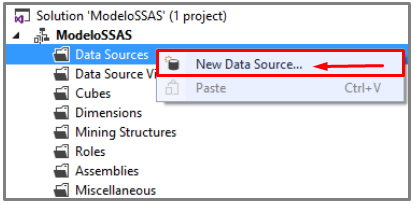
\includegraphics[width=8cm]{./Imagenes/img2}
	\end{center}

	\begin{center}
	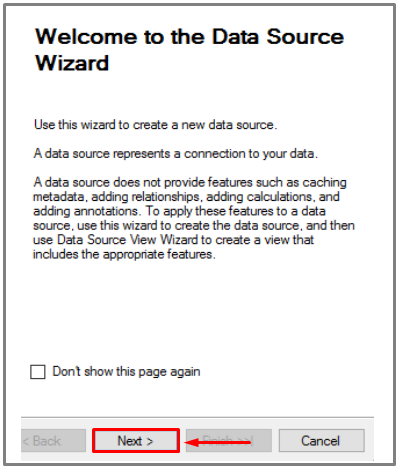
\includegraphics[width=8cm]{./Imagenes/img3}
	\end{center}	
	 \item Si es la primera vez que realizamos un proyecto de estos, no tendremos creadas conexiones. Click en New
para crear una nueva conexión hacia la base de datos Adventure Works DW:
	\begin{center}
	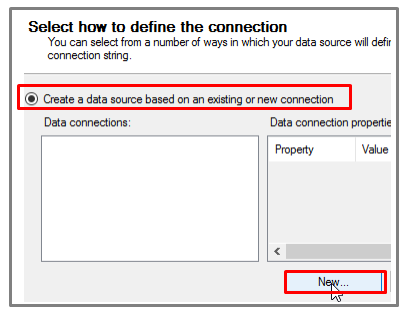
\includegraphics[width=8cm]{./Imagenes/img4}
    \end{center}	
	 \item Colocamos el nombre del Server donde se ubica la base de datos, en mi caso como es local coloco “.” ,
indicándole que es localhost. Ingresamos las credenciales y la base de datos Adventure Works DW 2014.
Luego Click en Ok:
	\begin{center}
	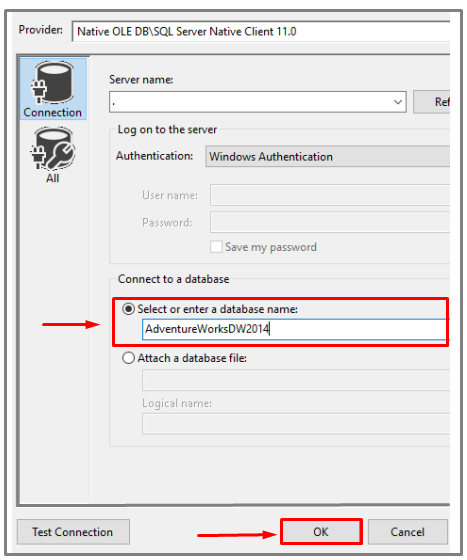
\includegraphics[width=8cm]{./Imagenes/img5}
    \end{center}	
	 \item Si todo está bien nos aparecerá la conexión creada en la sección de Data connections:
	\begin{center}
	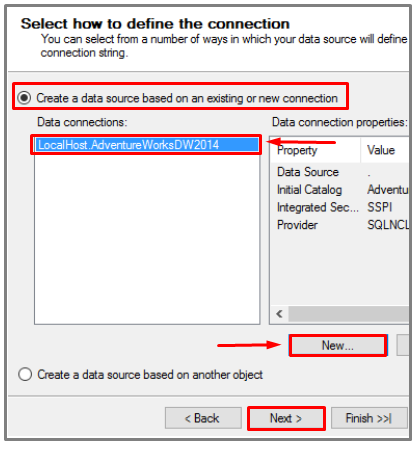
\includegraphics[width=8cm]{./Imagenes/img6}
    \end{center}	
	 \item En la ventana siguiente podemos definir las credenciales del Analysis Services y que utilizará para conectarse
al Data Source. En este caso utilizaremos las mismas credenciales del servicio. Para eso elegimos Use the
service account    
	\begin{center}
	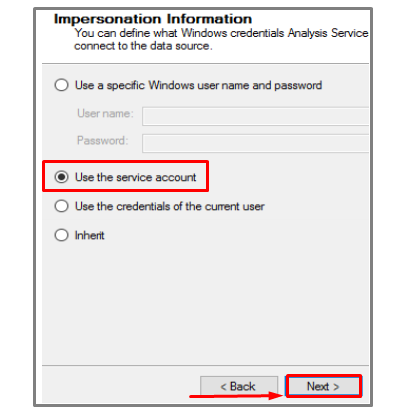
\includegraphics[width=8cm]{./Imagenes/img7}
    \end{center}
	 \item Colocamos un nombre para el Data Source y cen Finish:lick     
	\begin{center}
	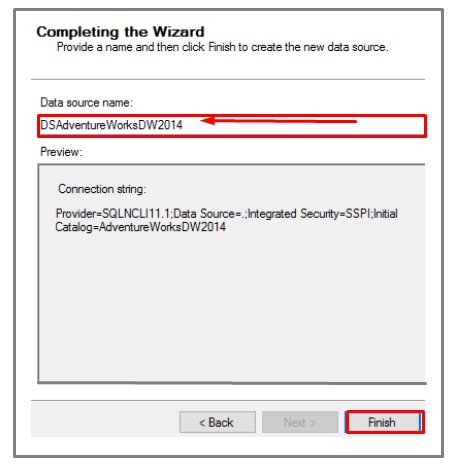
\includegraphics[width=8cm]{./Imagenes/img8}
    \end{center}	


\subsection{Creación de un Data Source View}

	 \item En el Solution Explorer nos ubicamos en Data Sources View y click derecho, seleccionando la opción de New Data Source View y se nos abrirá una ventana de resumen.
	\begin{center}
	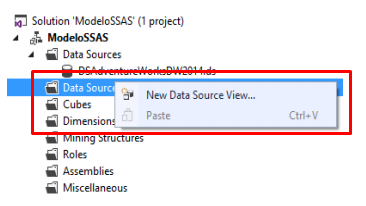
\includegraphics[width=8cm]{./Imagenes/img9}
	\end{center}	
\begin{center}
	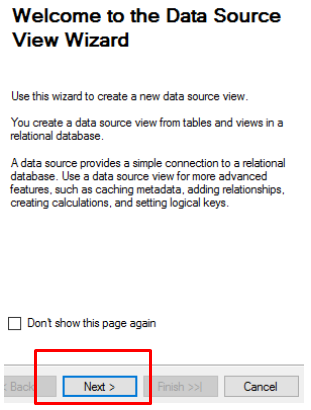
\includegraphics[width=8cm]{./Imagenes/img10}
\end{center}
	 \item Aquí nos aparecerán todos los Data Sources creados en la proyecto, en mi caso nos aparece el creado en
la sección 1.
\begin{center}
	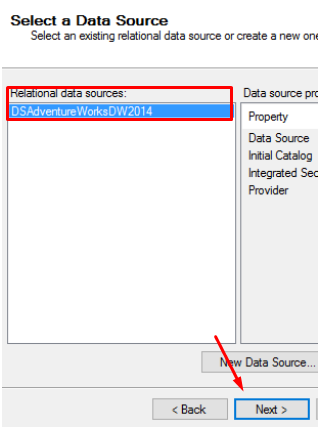
\includegraphics[width=8cm]{./Imagenes/img11}
\end{center}
	 \item Si bien es cierto hemos creado una conexión hacia Adventure Works DW, solo trabajaremos con algunas tablas. Seleccionamos las tablas DimDate,DimProduct y FactInternetSales:
\begin{center}
	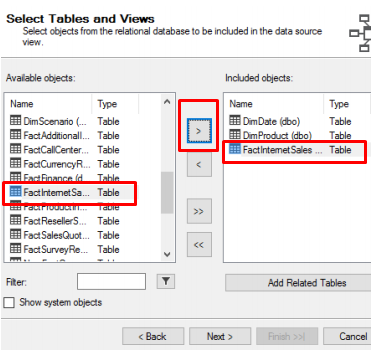
\includegraphics[width=8cm]{./Imagenes/img12}
\end{center}

	 \item Colocamos un nombre el Data Source View creado y click en Finish. Si todo va bien visualizaremos las tablas seleccionadas en el Data Source View:
\begin{center}
	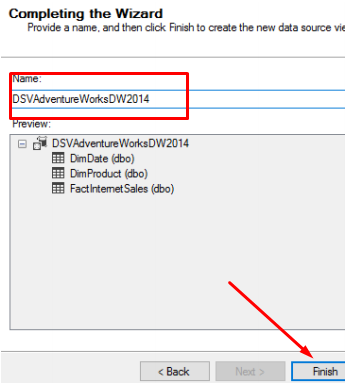
\includegraphics[width=8cm]{./Imagenes/img13}
\end{center}
\begin{center}
	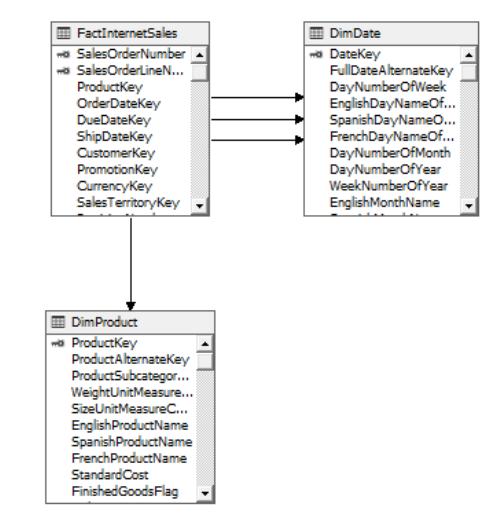
\includegraphics[width=8cm]{./Imagenes/img14}
\end{center}


\subsection{Creación de un Cubo}

	 \item En el Solution Explorer nos ubicamos en Cubes y click derecho, seleccionando la opción de New Cube. Se nos abrirá una ventana de resumen.
	\begin{center}
	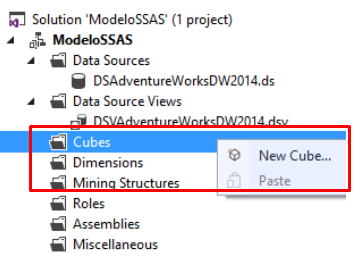
\includegraphics[width=8cm]{./Imagenes/img15}
	\end{center}
	 \item Para la creación de un cubo tenemos varias opciones. Use existing tables: Utilizar tablas del Data Source View. Create an empty cube: Crear un cubo vacío. En este caso utilizaremos las tablas seleccionadas en el Data Source View creada en la sección 2:
	\begin{center}
	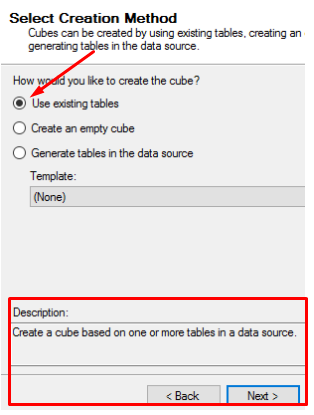
\includegraphics[width=8cm]{./Imagenes/img17}
	\end{center}
	 \item Aquí seleccionaremos la FactTable (Tablas de Hechos) , en este caso ubicamos FactInternetSales:
	\begin{center}
	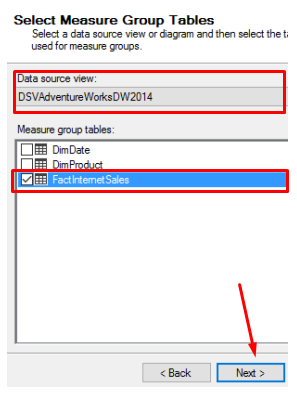
\includegraphics[width=8cm]{./Imagenes/img18}
	\end{center}	
	 \item Automáticamente el Data Tools identificará todos los campos numéricos y los marcará como candidatos a
ser medidas. Podemos observar que inclusive marca los campos utilizados como Foregin Keys. En este
caso, seleccionamos solo Order Quantity y Sales Amount:
	\begin{center}
	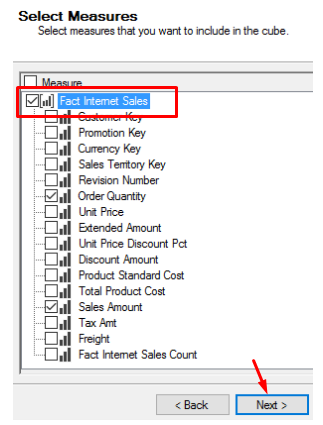
\includegraphics[width=8cm]{./Imagenes/img19}
	\end{center}	
	 \item Aquí seleccionamos las dimensiones por las cuales será analizada la data. Inclusive el Data Tools te indica
que podría tomar la misma FactTable como Dimensión. Seleccionamos Dim Date y Dim Product:
	\begin{center}
	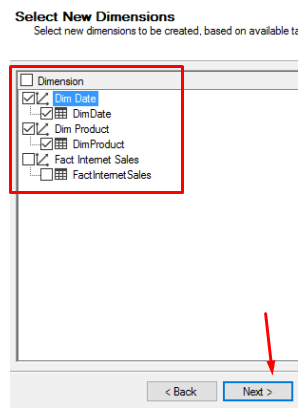
\includegraphics[width=8cm]{./Imagenes/img20}
	\end{center}
	 \item Colocamos un nombre el cubo:
	\begin{center}
	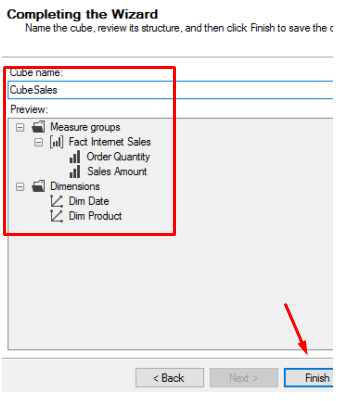
\includegraphics[width=8cm]{./Imagenes/img21}
	\end{center}	


\subsection{Proceso Cubo}

	 \item En el Solution Explorer nos ubicamos en el nuevo cubo creado CubeSales y click derecho, seleccionando la
opción de Process 
	\begin{center}
	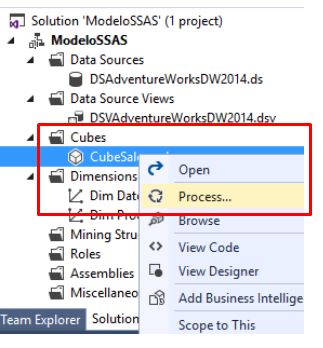
\includegraphics[width=8cm]{./Imagenes/img22}
	\end{center}	
	\begin{center}
	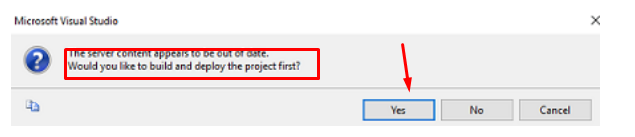
\includegraphics[width=8cm]{./Imagenes/img23}
	\end{center}	
	 \item En la nueva ventana seleccionamos la opción de Run…
	\begin{center}
	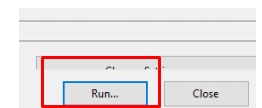
\includegraphics[width=8cm]{./Imagenes/img24}
	\end{center}
	\begin{center}
	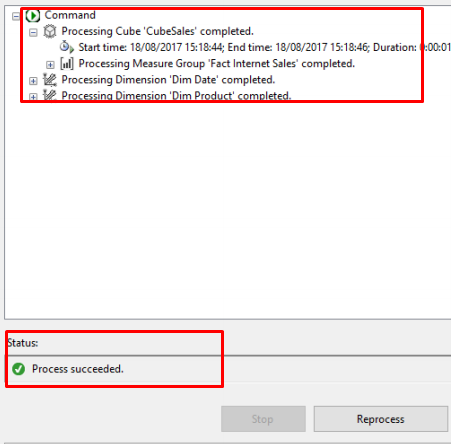
\includegraphics[width=8cm]{./Imagenes/img25}
	\end{center}	
	 \item Para verificar que nuestros datos se procesaron de forma correcta , en el cubo CubeSales nos dirigimos a la
pestaña de Browse:
	\begin{center}
	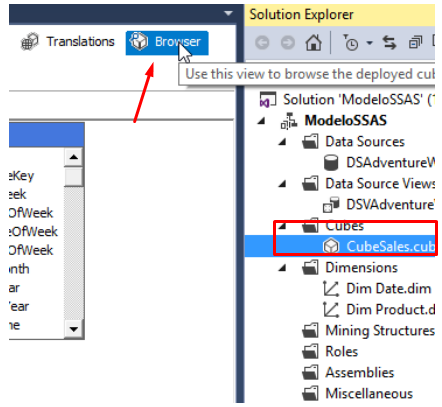
\includegraphics[width=8cm]{./Imagenes/img26}
	\end{center}	
	 \item En la pestaña de CubeSales, podemos tener un vistazo de las medidas y dimensiones. Arrastramos las
columnas de la Fact y la Dimensión Product obteniendo algo como:
	\begin{center}
	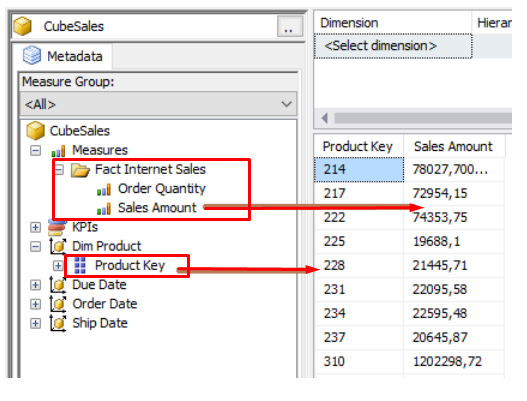
\includegraphics[width=8cm]{./Imagenes/img27}
	\end{center}	


\end{itemize}
		
\include{Secciones/Actividad05}

\end{document}
